\documentclass[11pt]{article}
\usepackage{geometry}                % See geometry.pdf to learn the layout options. There are lots.
\geometry{letterpaper}                   % ... or a4paper or a5paper or ... 
%\geometry{landscape}                % Activate for for rotated page geometry
%\usepackage[parfill]{parskip}    % Activate to begin paragraphs with an empty line rather than an indent
\usepackage{graphicx}
\usepackage{amssymb, amsmath}
\usepackage{epstopdf}
\usepackage[svgnames]{xcolor}
\usepackage{listings}
\DeclareMathOperator*{\argmax}{arg\,max}
\usepackage{placeins}

\lstset{language=R,
    basicstyle=\small\ttfamily,
    stringstyle=\color{DarkGreen},
    otherkeywords={0,1,2,3,4,5,6,7,8,9},
    morekeywords={TRUE,FALSE},
    deletekeywords={data,frame,length,as,character},
    keywordstyle=\color{blue},
    commentstyle=\color{DarkGreen},
    breaklines=true
}

\usepackage[hyphens]{url}
\usepackage{hyperref}

% own packages
\usepackage{float}
\usepackage{svg}
\usepackage{multirow}

\DeclareGraphicsRule{.tif}{png}{.png}{`convert #1 `dirname #1`/`basename #1 .tif`.png}

\title{Report II - SF2980 Risk Management \\
Group name: Risky Things}
\author{Khawla Gougas \and Maria Castaldo \and Stephan Tietz \and Marie Sergue \and Tomy Reguig}
\date{December 6th, 2018}                                           % Activate to display a given date or no date

\begin{document}
\maketitle


\section*{Project II a) -- Analyze both the bulk and the tails of a univariate distribution}
\subsection*{Objectives}

In this project you should find a univariate data set which you think is relevant from a risk management perspective. (This may include also non-financial contexts. Think of, for example, the construction of a dike or a bridge which has to stand up against extreme water levels, wind speeds, etc.) You should make sure that you have enough realizations for your data (50 being the minimum) which you can assume to be roughly i.i.d.\ 
\begin{itemize}
\item[(a)] Describe the data set, why you think it is interesting from a risk management perspective and try to find a suitable parametric distribution for the data set. Estimate necessary parameters by a suitable method and provide a goodness-of-fit analysis. 
\item[(b)] Describe the tail behavior of your distribution by the methods provided in the course. Is it reasonable to assume that your data has heavy tails? More general, is it reasonable to assume that the largest observations follow a generalized Pareto distribution? (Note: If you have found an interesting data set in (a) which has either less than 100 observations or seems not to follow a generalized Pareto distribution for its largest values, it may be advisable to choose a second data set.) Use the methodology described in Chapter 8.2.2 to estimate the $1-1/(2n)$-quantile of the distribution, where $n$ is the number of observations. 
\end{itemize}

\subsection*{Data}


For this exercise we use the sum of winter negative temperature data in Celsius as collected by Hipel and McLeod (1994). It contains yearly sums of negative temperatures from 1781 to 1988, a total of 208 measurements.
With environmental data one always has to consider seasonalities that make the iid assumption unlikely, but as this is yearly data we assume that no trends or seasonalities are present. One could argue about impact of climate change but we will neglect it for this task.

The right tail of this data (extremely cold years) could be interesting for a supplier of heating, that needs to buy and store oil reserves in autumn to supply people throughout the winter. Of course oil reserves should never run out so one needs to buy enough but on the other hand one doesn't want to buy too much as it would mean additional costs for storage over the next summer if it is not used up.

Figure \ref{fig:part1:raw_data} shows the data as is. It looks reasonably independent with no major trends visible. Figure \ref{fig:part1:hist_data} shows a seemingly right-skewed distribution with the right tail being heavier than the left tail.

Our data is bounded on the left side by 0, (no negative day in this year) and practically unbounded to the right (ignoring the physical limit of -273.15 degrees Celsius, where atoms stop moving).


\begin{figure}[!h]
 \center
  \def\svgwidth{0.7\columnwidth}
  \includesvg{img/raw_data.svg}
  \caption{Sum of negative temperatures per year from 1781 to 1988.}
  \label{fig:part1:raw_data}
\end{figure}

\begin{figure}[!h]
 \center
  \def\svgwidth{0.7\columnwidth}
  \includesvg{img/hist_data_mean_median.svg}
  \caption{Historgram of the temperature data. Mean is shown in red and median in blue. The distribution seems to be skewed to the right with a heavy right tail.}
  \label{fig:part1:hist_data}
\end{figure}

\subsection*{Mathematical Background}

As our observations belong to $\mathbb{R}$ we have considered the following distributions to fit the data:
\begin{itemize}
    \item \textbf{Chi-squared distribution}, which has probability density function
    \[
    f(x;k) = \begin{cases}
    \frac{x^{\frac{k}{2}-1}e^{-\frac{x}{2}}}{2^{\frac{k}{2}}\Gamma(\frac{k}{2})} \;\;\;\text{if} x>0\\
    0, \;\;\;\;\;\;\; x\leq 0
    \end{cases}
    \]
    where $\Gamma(k/2)$ denotes the gamma function. 
    It starts from 0 and is skewed to the right, so it might be a good choice for our data.
    \item \textbf{Weibull distribution}
    which has probability density function
    \[
    f(x;\lambda,k) = \begin{cases}
    \frac{x}{\lambda}\left(\frac{x}{\lambda}\right)^{k-1}e^{-(x/\lambda)^k} x>0\\
    0, \;\;\;\;\;\;\; x\leq 0
    \end{cases}
    \]
    Just like the Chi-Squared it does not allow negative values. It can be asymmetric and right skewed, so it is a likely candidate for our dataset. 
    
    \item \textbf{Exponential distribution} which has probability density function
    \[
    f(x;\lambda) = \begin{cases}
    \lambda e^{-\lambda x},\;\;\; x>0\\
    0, \;\;\;\;\;\;\; x\leq 0
    \end{cases}
    \]
    As this distribution is monotonically decreasing we don't expect it to model well our data on the first observations (left tail) but it might well approximate the right tail.
    
    \item \textbf{Normal distribution} which has probability density function
    \[
    f(x; \mu, \sigma) = \frac{1}{\sqrt{2\pi \sigma^2}}\exp{-\frac{(x-\mu)^2}{2\sigma^2}}
    \]
    The normal is symmetric around it's mean and allows infinitely big or small values and therefore also negative values, which are not possible in our dataset. We assume it will not be a good choice for our data but keep it for comparison.
    
    
\end{itemize}


\textbf{Optimisation:} All parameters are fitted using maximum likelihood estimators. For the normal and exponential the closed form of the ML estimate was used, for the others downhill methods were used.

Assuming our timeseries $X_1$ to $X_n$ comes from the distribution family $F$, we want to maximise the likelihood of the parameters given the data.
$$
\max_{\theta} P(\theta | X) = \max_{\theta} \prod_{i=1}^{n} f_\theta(X_i)
$$

$$
\hat{\theta} = \argmax_{\theta} P(\theta | X)
$$

\textbf{Tail analysis:} We again used the ML Estimator as described above to find values for the generalized Pareto Distribution. From the parameters of the gPD conclusions over the tail behaviour can be drawn:

\begin{itemize}


    \item \textbf{Generalized Pareto distribution}
    with probability density function
    \[
     G(x;\gamma, \beta) = 1-(1+\gamma x/\beta)^{-1/\gamma}\;\;\;\;\; \text{for } x \geq 0
    \]
    This distribution has been used to model the right tail and study its heaviness.
    
    
\end{itemize}


\subsubsection*{Implementation}



\begin{lstlisting}

library(stats4)
library(MASS)
library(gPdtest)
library(ggplot2)

data = read.csv('winter-negative-temperature-sum-.csv')
vals = as.matrix(data[,2])

n = length(vals)

# Plot the time series
data_overview = data.frame(year=data[,1], temp=data[,2])

# Plot histogram, mean and median
ggplot(data_overview, aes(x=year, y=temp)) + geom_line()
(ggplot(data_overview, aes(x=temp)) 
  + geom_histogram()
  + geom_vline(xintercept = mean(vals), col="Red")
  + geom_vline(xintercept = median(vals), col="Blue"))


################# FIT DIFFERENT DISTRIBUTIONS #######################

# Scale the values for fitting the Chi Square,
#doesn't impact the other distributions
vals = vals/35

# Fit a normal around the data
fittednorm = fitdistr(vals, "normal")$estimate
qqplot(qnorm((n-seq(1,n)+1)/(n+1))*fittednorm[2]+fittednorm[1], vals,
ylab="Empirical Quantiles", xlab="Normal Quantiles")
abline(0,1)

# Fit an exponential around the data
fittedexp = fitdistr(vals, "exponential")$estimate
qqplot(qexp((n-seq(1,n)+1)/(n+1), rate=fittedexp[1]), vals,
ylab="Empirical Quantiles", xlab="Exponential Quantiles")
qqline(vals, distribution = function(q){qexp(q,rate=fittedexp[1])})

# Fit a weibull around the data
fittedw<-fitdistr(vals, "weibull")$estimate
qqplot(qweibull((n-seq(1,n)+1)/(n+1),shape=fittedw[1], scale=fittedw[2]), vals, ylab="Empirical Quantiles", xlab="Weibull Quantiles")
abline(0,1)

# Fit a chi square around the data
fittedchi<-fitdistr(vals, "chi-squared", start=list(df=2))$estimate
qqplot(qchisq((n-seq(1,n)+1)/(n+1), df=fittedchi[1]), vals, ylab="Empirical Quantiles", xlab="Chi-Square quantiles")
abline(0,1)


# Plot a histogram and the different theoretical distributions
x = seq(0,30, length=100)
hist(vals, freq=FALSE, breaks=20)
lines(x,dchisq(x, df=fittedchi[1]), col='green')
lines(x,dweibull(x, shape=fittedw[1], scale=fittedw[2]), col='blue')
lines(x,dnorm(x, mean=fittednorm[1], sd=fittednorm[2]), col='red')
lines(x,dexp(x, rate=fittedexp[1]), col='yellow')

\end{lstlisting}

To analyze the right tail of the dataset the following code hase been used. Libraries \textbf{ismev} and \textbf{evir} have been used.
\begin{lstlisting}
#going back to non-rescaled values
vals = 35*vals

par(mar=c(2,2,2,2))
#plotting the confidence intervals for paratemters of fittend 
#GPD changing the threshold
gpd.fitrange(vals, umin=300, umax=550)
title("Confidence interval for shape and scale varying threshold")
#considering this plot and the size our sample we decide to cut in 380
my_threshold = 380

ecdf(vals)(my_threshold)
#the percentage of dataset above the threshold is the 20%
my_gpd<-gpd(vals,my_threshold)
my_gpd$par.ests

#Save the parameters obtained with maximum likelihood
gamma = my_gpd$par.ests[1]
beta  = my_gpd$par.ests[2]

#let us evaluate the goodness of fit with a q-q plot
qplot(vals, threshold=my_threshold,gamma)

#plot the distribution over the histogram of the tail
x = seq(0,max(vals)-my_threshold, length=100)
hist(vals[vals>my_threshold], freq=FALSE,+
    breaks=seq(my_threshold,780,30), main="Histogram of values over threshold", legend="GPD approximation")
lines(x+my_threshold,dGPD(x, gamma, beta), col='green')
\end{lstlisting}

Using the generalized Pareto distribution fitted with the script above, the quantile of $1-1/2n$, where n is the number of observations in the dataset, has been obtained with the following implementation
\begin{lstlisting}
#evaluation of quantile
n = length(vals)
p = 1-1/(2*n)
my_p = -((1-p)*length(vals)/length(vals[vals>my_threshold])-1);
quantile_p = my_threshold+qGPD(my_p,gamma,beta)
#the empirical closest quantile we have is:
quantile(vals, p)
\end{lstlisting}


\subsection*{Results}

Parameters of the theoretical distributions are found with Maximum Likelihood Estimates and can be seen in the following table:
\begin{table}[H]
\centering
\begin{tabular}{lll}
                                 & \textbf{Parameter} & \textbf{Value} \\
\hline
\multirow{2}{*}{\textbf{Normal}} & Mean               & 276.0529       \\
                                 & Variance           & 134.2459       \\
\hline
\textbf{Exponential}                      & Rate               & 0.00362        \\
\hline
\textbf{Weibull}                          & Shape              & 2.1854         \\
                                 & Scale              & 312.6239       \\
\hline
\textbf{Chi Square}                       & Scaling            & 0.0286         \\
                                 & Degree             & 7.9375        \\
\hline
\end{tabular}
\caption{Optimal parameters for different distribution families obtained by ML estimate.}
\end{table}

\begin{figure}[H]
\centering
\subfloat{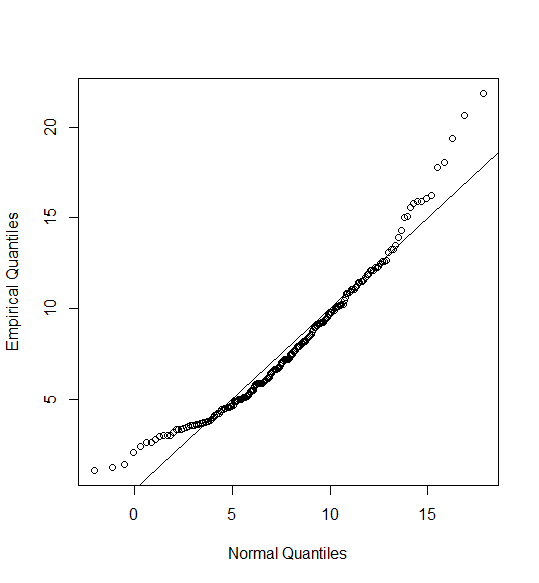
\includegraphics[width = 0.35\textwidth]{img/qq_normal.png}} 
\subfloat{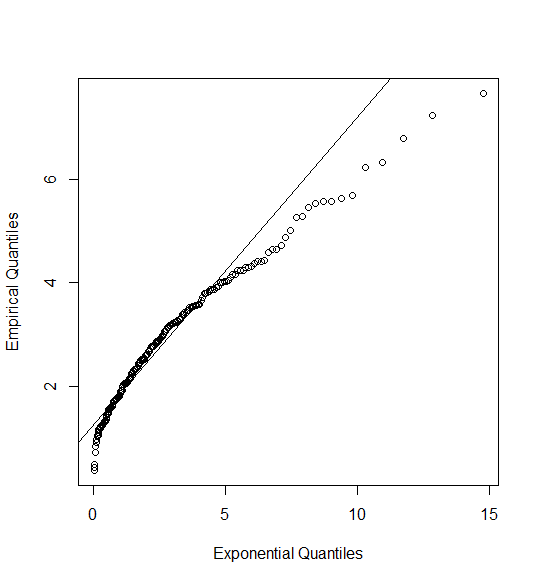
\includegraphics[width = 0.35\textwidth]{img/qq_exp.png}}\\
\subfloat{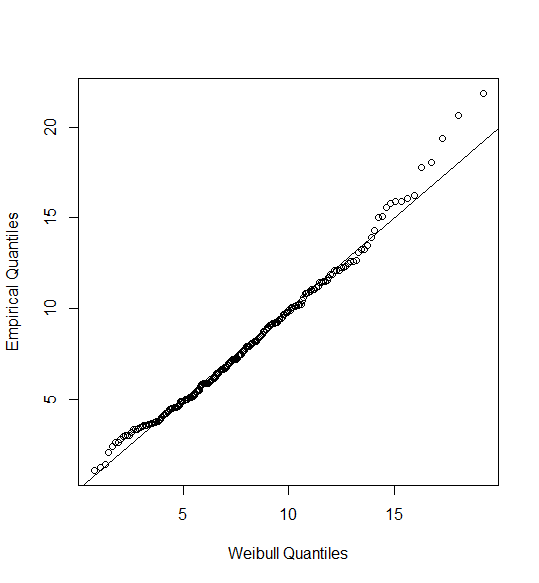
\includegraphics[width = 0.35\textwidth] {img/qq_weibull.png}}
\subfloat{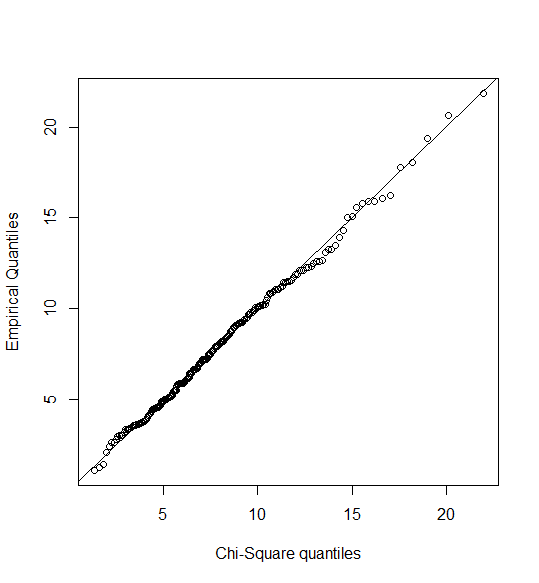
\includegraphics[width = 0.35\textwidth]{img/qq_chi.png}} 
\caption{The empirical distribution quantiles against different distributions. Parameters have been fitted with MLE, for distributions without scale parameter the data has been scaled before fitting.}
\label{fig:part1:qq_plots}
\end{figure}

Figure \ref{fig:part1:qq_plots} shows QQ plots of the the empirical distributions vs several theoretical distributions. 

Clearly the normal distribution (top left) is not a good fit. The left tail is too heavy, the right tail too light. This comes as no surprise, as we have already seen that the emp. dist is left bounded, skewed and heavier tailed on the right side.

The exponential distribution (top right) fails to model the left tail, as it doesn't start from 0 but is continuously decreasing instead. Early on it's right tail is too heavy to model the emp. distribution.

The Weibull distribution mostly gives a pretty decent fit, especially the left tail is much better than for the previous distributions, unfortunately the right tail seems to not be heavy enough. 

Lastly the Chi Square distributions describes the data in almost perfect manner. Both the left and the right tail are very close to the vertical line with only minor oscillations. No clear trend towards either distribution are visible.

Figure \ref{fig:part1:fitted_hist} shows the histogram of the (scaled by $1/35$) data with the PDFs of the fitted Normal, Weibull and Chi Square.
Both the Weibull and the Chi Square reasonably explain most of the data. The Chi Square captures the drastic increase in probability mass in the left tail and the slow fade out in the right tail slightly better than the Weibull.







\begin{figure}[!ht]
 \center
  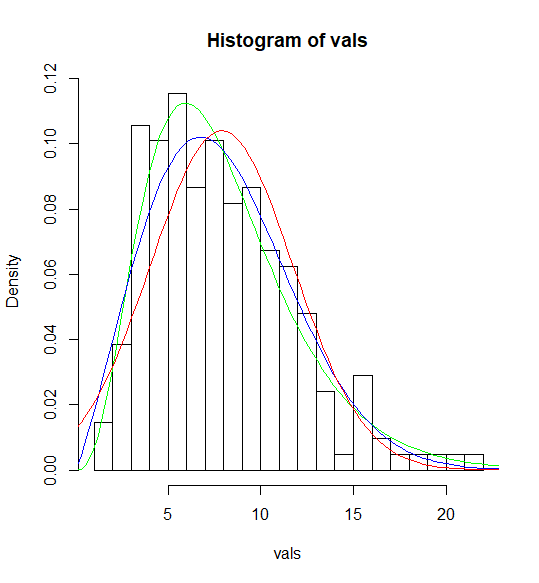
\includegraphics[width = 0.5\textwidth]{img/hist_chi_weibull.png}
  \caption{Empirical distribution with fitted Normal (red), Weibull (blue) and Chi Square (green) PDFs. The Chi Square best models the quick gain in mass from 0 to 5 and the long tail in the range of 15 to 25.}
  \label{fig:part1:fitted_hist}
\end{figure}

\FloatBarrier
\subsubsection*{Right Tail Model}
Let us now focus on the behavior of the right tail. In order to establish which threshold to consider for this study, two plots have been generated (Figure \ref{miaFigura1}) showing maximum likelihood estimates and confidence intervals of the shape and modified
scale parameters over a range of threshold. The aim is to choose a threshold which still grants small confidence intervals for the parameters. As our data set has not got many observations, a threshold of 380 can be considered a good compromise to not include too many observations and to still not have wide confidence intervals.

\begin{figure}[!h]
 \center
  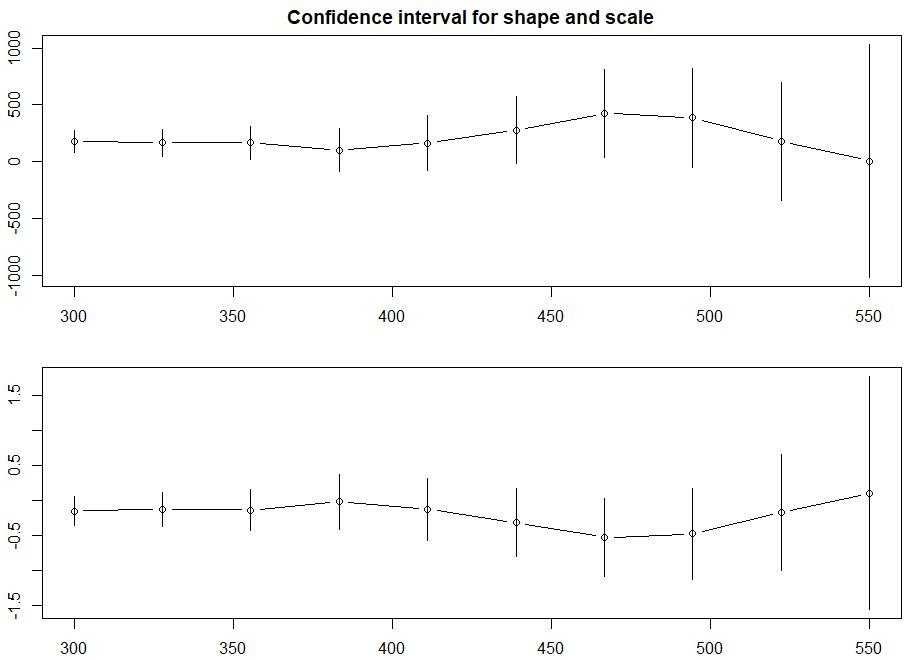
\includegraphics[scale = 0.3]{miaFigura1.JPG}
  \caption{Maximum likelihood estimates and confidence intervals of the shape and modified
scale parameters over a range of threshold}
  \label{miaFigura1}
\end{figure}

Using a threshold equal to $380$ we fitted a generalized Pareto distribution evaluating the parameters $\beta$ and $\gamma$ by maximum likelihood. The values obtained are
$$
\gamma = -0.034 \;\;\;\;\;\;\;\;\;\;\;\; \beta = 99.518.
$$
As $\gamma$ is smaller than zero, the tail considered is presumably a light tail. It should be noted though that the confidence interval for $\gamma$ at 380 reaches into the positive realm, so this is not very strong evidence.

Figure \ref{miaFigura2} compares the empirical distribution of our data set with the fitted one while \ref{miaFigura3} shows the Q-Q plot of the empirical and theoretical quantiles obtained fitting the generalized Pareto distribution by maximum likelihood.
\begin{figure}[!h]
 \center
  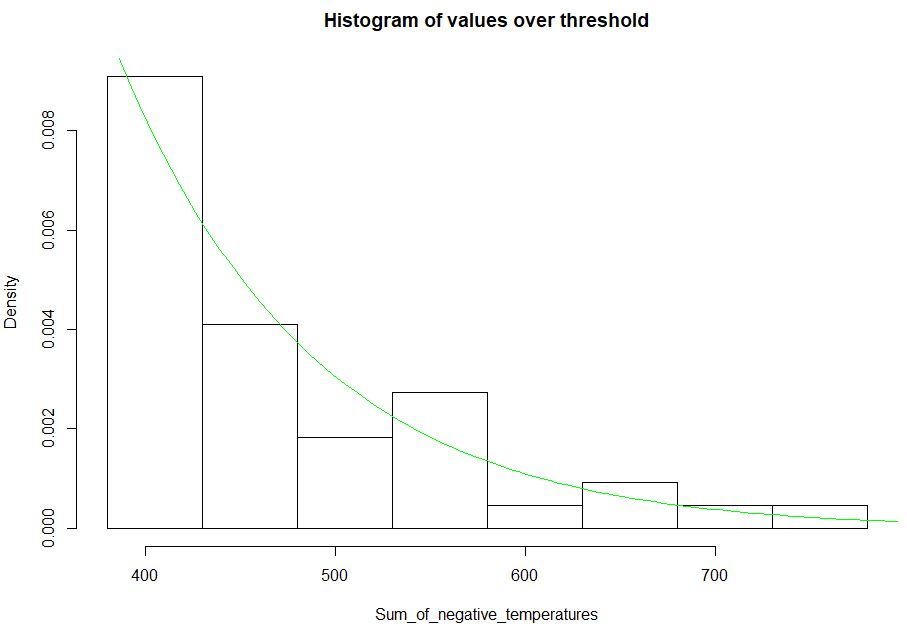
\includegraphics[scale = 0.3]{miaFigura2.JPG}
  \caption{Histogram of the values over threshold and density function of the fitted generalized Pareto distribution}
  \label{miaFigura2}
\end{figure}
\begin{figure}[!h]
 \center
  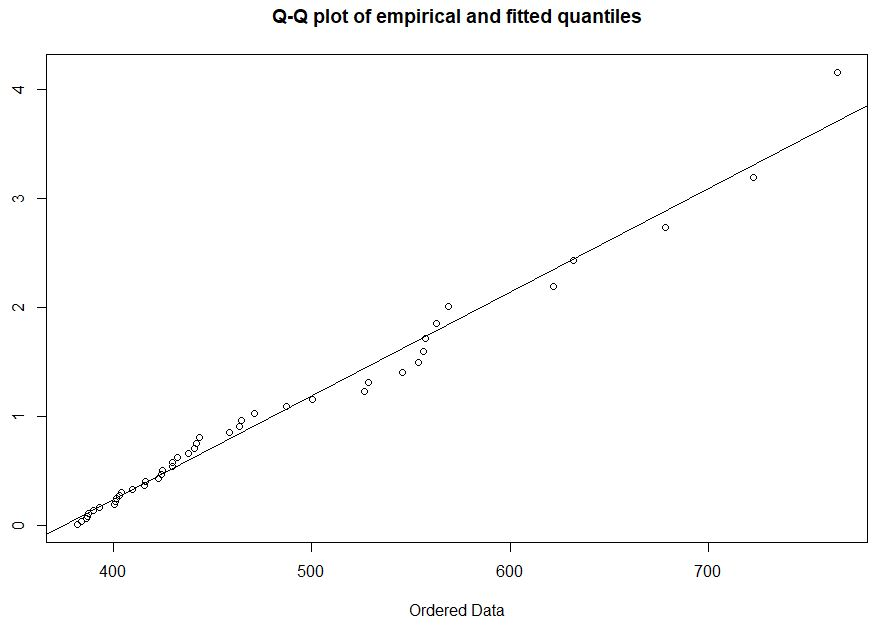
\includegraphics[scale = 0.3]{miaFigura3.JPG}
  \caption{Q-Q plot of the empirical and thoretical quantiles from the fitted generalized Pareto distribution}
  \label{miaFigura3}
\end{figure}
As both Figure \ref{miaFigura2} and \ref{miaFigura3} show, it seams reasonable to use a Generalized Pareto distribution to approximate the behavior of the largest observation. The histogram seems well approximated by our fitting and also the biggest quantile show to be on the diagonal of the Q-Q plot.


Using the fitted distribution above the quantile in $1-\frac{1}{2n} = 99.76\%$, where $n$ is the number of observations, the quantile can be approximated by
\[
\hat F_{GPD}^{-1}(1-\frac{1}{2n}) = 793.13
\]
which is quite reasonable as the greatest value observed in the data set is 764.9 and, as the number of unique observations we have is 208, it would be the empirical approximation of the 100\% quantile.

\subsection*{Summary}


We conclude that a Chi Square distribution models this temperature data best. With it's asymmetric behaviour it fits the data reasonably good in the center and on both tails of the distribution. 

We specifically analyzed the right tail of the distribution and found it to be heavier tailed than the normal distribution but still generally light tailed. 
Fitting the tail with a generalized Pareto distribution we get a negative value for the parameter $\gamma$. This means the distribution is bounded which is a reasonable assumption as we expect low temperatures to be bounded too.

The heating company can expect that the sum of negative temperatures will not be above 793.13 Celsius in  99.76\% of years.
\pagebreak

\section*{Project II b) -- Analyze dependence structures}

\subsection*{Objectives}
In this project you should find a bivariate data set $(X_i, Y_i)_{1 \leq i \leq n}$ which you think is relevant from a risk management perspective (this could be, for example, log-returns of two different stocks, but it is very welcome to think a bit out of the box again). You should make sure that you have enough realizations for your data (50 being the minimum but the more the better) which you can assume to be roughly i.i.d.\ 
\begin{itemize}
\item[(a)] Describe the data set, why you think it is interesting from a risk management perspective and try to describe the dependence structure by deriving the dependence measures which we discussed in the course (correlation, Kendall's tau, ...). Is the dependence structure strong or weak? Do the tails have a different dependence structure than the rest of the distribution?
\item[(b)] Transform the data set such that both marginal distributions are approximately uniform on $[0,1]$ (this can be done by looking at $(F_{n,X}(X_i), F_{n,Y}(Y_i))_{1 \leq i \leq n}$, where $F_{n, X}$ and $F_{n,Y}$ are the empirical distribution functions derived from the $(X_i)_{1 \leq i \leq n }$ and $(Y_i)_{1 \leq i \leq n }$, respectively). Try to find a copula to model the transformed bivariate distribution. Assess the goodness of fit. Use the fitted copula to evaluate (via simulation) the probability that $P(X>F_X^{-1}(1-1/n), Y>F_Y^{-1}(1-1/n))$ (where $(X,Y)$ has the same distribution as any of your original observations and $F_X$ and $F_Y$ are their corresponding marginal distributions) or a similar extreme event which you deem relevant for your data set. 
\end{itemize}

\subsection*{Mathematical Background}
({\it Instructions: provide a mathematical background by briefly explaining the dependence measures that you used and the chosen family of copulas. Describe how the probability you are looking for can be evaluated via simulation})

There are multiple ways to measure dependence of random variables. In this exercise we will mainly use the following two methods:
\begin{itemize}
    \item \textbf{Correlation coefficient}: $Corr(X,Y) = \rho(X,Y) = \frac{Cov(X,Y)}{\sqrt{Var(X)Var(Y)}} \in [-1;1]$
    This is just the well know correlation coefficient for linear correlation.
    \item \textbf{Kendall's $\tau$}: $$\tau(X,Y) = P((X-X^{'})(Y-Y^{'})>0) - P((X-X^{'})(Y-Y^{'})<0)$$
    We can estimate Kendall's $\tau$ by : $$\hat{\tau} = \binom{n}{2}^{-1}\sum_{i=1}^{n}\sum_{j=1}^{i}sign((X_{i}-X_{j})(Y_{i}-Y_{j})) \in [-1;1]$$
    It's advantage over the simple correlation coefficient is that it is invariant to any monotonically increasing nonlinear transformations of the data.
\end{itemize}

The copulas investigated are the normal copula, the student t copula and the Clayton copula. With R being the linear correlation matrix their d-dimensional distribution functions are given by:
\begin{itemize}
    \item \textbf{Normal copula}: 
    $$C_{R}^{GA} = P(\Phi(X_1) \leq u_1, ..., \Phi(X_d) \leq u_d) = \Phi_{R}^{d}(\Phi^{-1}(u_1), ..., \Phi^{-1}(u_d) )
    $$ with X having a $N_d(0,R)$ distribution.
    \item \textbf{Student-t copula}: 
    $$
    C^{t}_{\nu,R} = P(t_\nu(X_1) \leq u_1, ... t_\nu(X_d) \leq u_d ) = t^{d}_{\nu,R}(t^{-1}(u_1), ..., t^{-1}(u_d))
    $$ with X having a $t_d(0,R,\nu)$ distribution.
    \item \textbf{Clayton copula}:
    $$
    C_{\Theta}^{Cl} = (u_1^{-\Theta} + ... + u_d^{-\Theta} - d +1)^{-1/\Theta}
    $$ with X having a $Gamma(1/\Theta,1)$ distribution.
\end{itemize}

We chose these copulas as they are well studied and especially the student-t copula is a good guess for log stock returns.

\subsection*{Results}

\begin{lstlisting}
X <- read.csv("individual_stocks_5yr\\ADBE_data.csv")
Y <- read.csv('individual_stocks_5yr\\ADSK_data.csv')
\end{lstlisting}
We will compare the log returns of the opening stock prices of two stocks that are part of the S&P500 index
\begin{lstlisting}
X <- X[,2]
Y <- Y[,2]
X <- diff(log(X))
Y <- diff(log(Y))
\end{lstlisting}
Scatter plot to have a first quick look into the data and have an idea if they are more or less correlated 
\begin{lstlisting}
scatter.smooth(x=X, y=Y, main="Y ~ X")
\end{lstlisting}
\begin{figure}[!ht]
 \center
  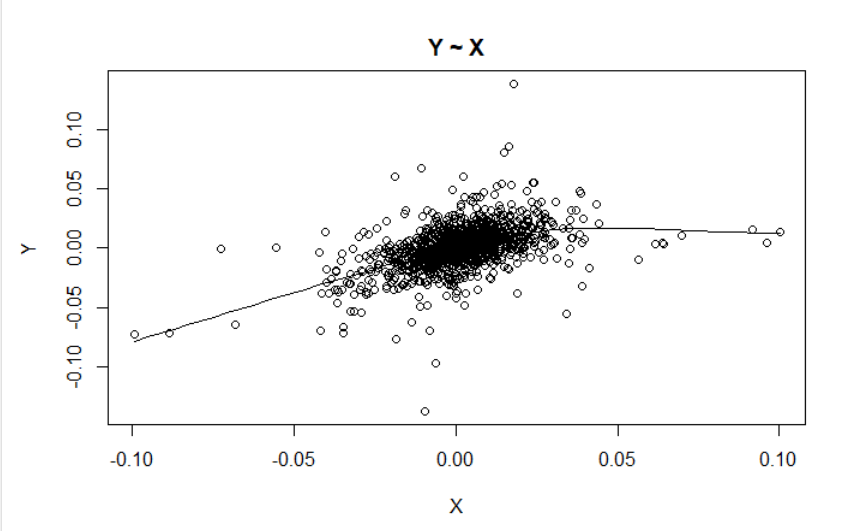
\includegraphics[width=\linewidth]{img/scatter_plot.PNG}
  \caption{Scatter plot between the log return of the two stocks (ADBE, ADSK)}
  \label{fig:plot data}
\end{figure}
\begin{lstlisting}
Rho <- function(X,Y){
  reg <- lm(Y~X)
  reg_sum <- summary(reg)
  return(reg_sum$r.squared)
}
Rho(X,Y)
[1] 0.2275917
\end{lstlisting}
We assumed a simple model which is a linear regression between our 2 data sets, which means $Y_{i} = a + \rho X_{i} + \epsilon_{i}$  $\forall i$
The linear regression model between our 2 data sets gives a r-squared quite low (square of the correlation coefficient), $\rho ^{2} = 0.228$. Which means that $\pho$ the correlation coefficient is $\rho = \pm0.447$. 
With that value of $\rho$ being significantly greater than $0$, we can think that the 2 data sets are correlated.  

Let's now have a look  at Kendall's Tau
\begin{lstlisting}
Tau <- function(X,Y){
  tau = 0
  for (i in 1:length(X)){
    for (j in 1:i){
      tau = tau + sign((X[i]-X[j])*(Y[i] - Y[j]))
    }
  }
  tau = (1/choose(length(X),2))*tau
  return(tau)
}
Tau(X,Y)
[1] 0.3694908
\end{lstlisting}
After computation, we find an empirical Kendall's $\tau$ of $0.369$, which is positive and significantly different from zero. That means that our pairs of observations are often concordant. 

This way we see that the Kendall's $\tau$ gives the same interpretation than the correlation coefficient. We can conclude that the dependence structure between our two stocks is pretty strong.


To strengthen our conclusion, let's have a look at the regression between the stock price directly, without taking the log returns.
\begin{lstlisting}
S_1 <- read.csv("individual_stocks_5yr\\ADBE_data.csv")
S_2 <- read.csv('individual_stocks_5yr\\ADSK_data.csv')
S_1 <- S_1[,2]
S_2<- S_2[,2]
Rho(S_1, S_2)
[1] 0.9134792
scatter.smooth(x=S_1, y=S_2, main="Y ~ X")
\end{lstlisting}
\begin{figure}[!ht]
 \center
  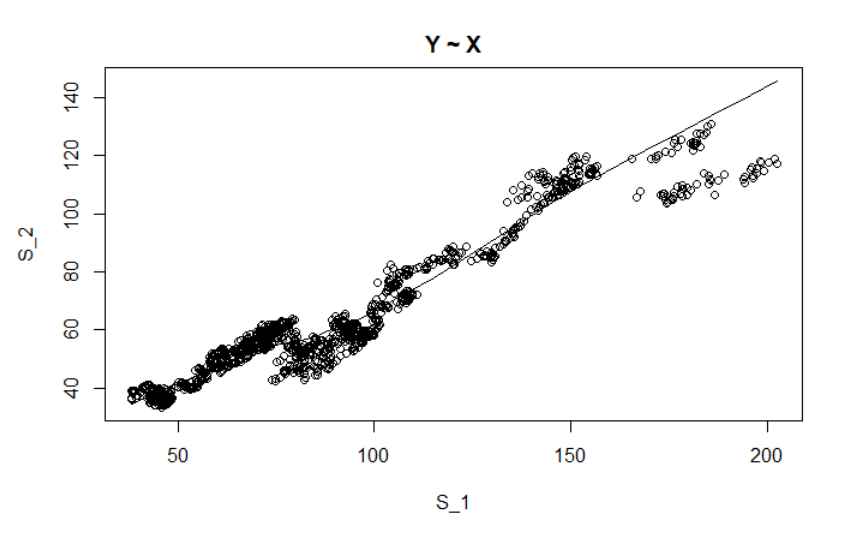
\includegraphics[width=\linewidth]{img/scatter_plot2.PNG}
  \caption{Scatter plot between the  prices of the two stocks (ADBE, ADSK)}
  \label{fig:plot data}
\end{figure}
\pagebreak
The linear regression model between the 2 stock prices gives a r-squared this time really high, $\rho ^{2} = 0.913$. Which means that $\pho$ the correlation coefficient is $\rho = 0.956$. 
With that value of $\rho$ being high, we will keep our first conclusion that the 2 data sets are correlated.


Tails dependance structure
\begin{lstlisting}
X_sorted = sort(X)
Y_sorted = sort(Y)
X_lower = X_sorted[1:floor(0.025*length(X))]
Y_lower = Y_sorted[1:floor(0.025*length(Y))]
X_upper = X_sorted[(floor(0.975*length(X))+1):length(X)]
Y_upper = Y_sorted[(floor(0.975*length(Y))+1):length(Y)]

rho_lower = Rho(X_lower, Y_lower)
rho_upper = Rho(X_upper, Y_upper)
rho_lower
rho_upper
[1] 0.8256243
[1] 0.829635
\end{lstlisting}
When we compute the correlation coefficient for the $2.5\%$ ($5\%$ of the total observations) lowest and largest log returns between our observations.
We come up with 2 correlations coefficient pretty high, this way we also want to conclude that the tails have also a dependence structure.


To verify our idea we use a scatter plot
\begin{lstlisting}
par(mfrow=c(1,2))
scatter.smooth(x=X_lower, y=Y_lower, main="Y ~ X")
scatter.smooth(x=X_upper, y=Y_upper, main="Y ~ X")
\end{lstlisting}
\begin{figure}[!ht]
 \center
  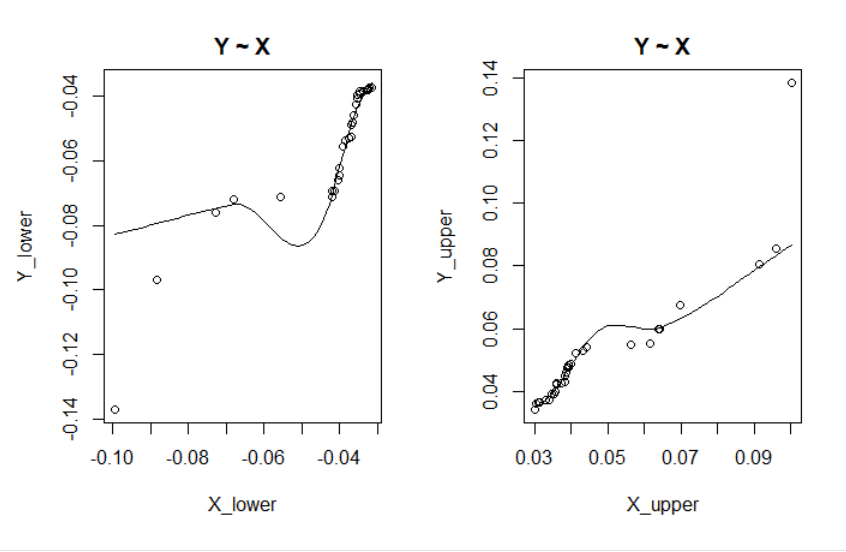
\includegraphics[width=\linewidth]{img/scatter_plot3.PNG}
  \caption{Scatter plot between the  prices of the two stocks (ADBE, ADSK)}
  \label{fig:plot data}
\end{figure}
On the plots we see that most of our extreme observations are nicely correlated, that the regression could be linear. 
However for the very extreme observations, we see that the regression is not linear anymore and so the it seems like the very extreme observations are not completely correlated, or at least not as much as for the rest of the observations.


Let's compute again the correlation coefficient but this time for $1\%$ of the total observations

\begin{lstlisting}
X_sorted = sort(X)
Y_sorted = sort(Y)
X_lower = X_sorted[1:floor(0.005*length(X))]
Y_lower = Y_sorted[1:floor(0.005*length(Y))]
X_upper = X_sorted[(floor(0.995*length(X))+1):length(X)]
Y_upper = Y_sorted[(floor(0.995*length(Y))+1):length(Y)]

rho_lower = Rho(X_lower, Y_lower)
rho_upper = Rho(X_upper, Y_upper)
rho_lower
rho_upper
[1] 0.713547
[1] 0.706529
\end{lstlisting}
We again come up with 2 correlations coefficient quite high, though lower than the previous ones. This way we also conclude that the tails have a depedence structure.


\begin{lstlisting}
library(psych)
library(MASS)
library(fitdistrplus)
#import the stock data from the csv file
stocks1 = read.csv("ADBE_data.csv",header=TRUE,sep=",")$high
stocks2 = read.csv("ADSK_data.csv",header=TRUE,sep=",")$high
#calculate the log returns
stocks1 <- diff(log(stocks1))
stocks2 <- diff(log(stocks2))
#make a data frame composed of both stocks
data = cbind.data.frame(stocks1,stocks2)
data <- as.matrix(data)
plot(data)
#fit the first maginal to a uniform distribution on [0,1]
fitdata1 <- fitdist(stocks1, "unif",method="mge", gof="CvM")
summary(fitdata1)
plot(fitdata1)
#fit the first maginal to a uniform distribution on [0,1]
fitdata2 <- fitdist(stocks2, "unif",method="mge", gof="CvM")
summary(fitdata2)
plot(fitdata2)

#TEST

#the copula is the distribution function of a random vector U whose components U_k are uniformly
#distributed on [0,1] 

Estimate_stocks1<-pobs(stocks1)
Estimate_stocks2<-pobs(stocks2)
plot(Estimate_stocks1, Estimate_stocks2)
# Fit a Student-t-copula
currfit<-fitCopula(tCopula(),cbind(Estimate_stocks1, Estimate_stocks2))
pairsRosenblatt(pairwiseCcop(cbind(Estimate_stocks1, Estimate_stocks2), tCopula(0.75, df=8.89)))
\end{lstlisting}
\begin{figure}[!ht]
 \center
  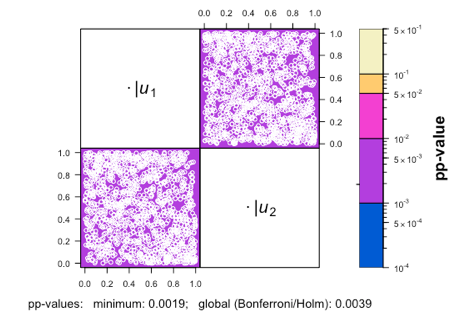
\includegraphics[width=70mm]{Student_t}
  \caption{Student t copula}
  \label{fig:plot data}
\end{figure}
It seems that the Student-t copula doesn't fit the data very well.
We will try it again with a normal copula.
\begin{lstlisting}
# Fit a Normal-copula
currfit <- fitCopula(normalCopula(),cbind(Estimate_stocks1,Estimate_stocks2))
pairsRosenblatt(pairwiseCcop(cbind(Estimate_stocks1,Estimate_stocks2),normalCopula(0.53)))
\end{lstlisting}
\begin{figure}[!ht]
 \center
  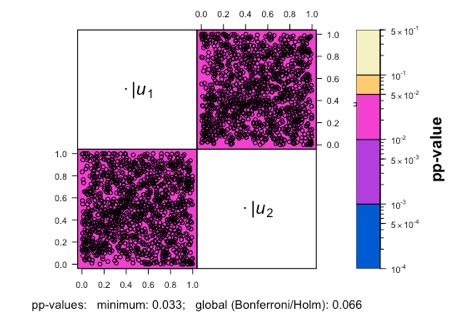
\includegraphics[width=70mm]{Normal}
  \caption{Normal copula}
  \label{fig:plot data}
\end{figure}
\pagebreak
The Normal copula doesn't fit either.
We will use the package VineCopula and the function BiCopSelect to find the best copula to fit our data. It uses a Maximum Likelihood approach to estimate the parameters of a lot of different bivariate copulas.
\begin{lstlisting}
selectedCopula <- BiCopSelect(Estimate_stocks1,Estimate_stocks2,familyset=NA)
selectedCopula
\end{lstlisting}
The function suggest to use a Student-t copula.
We fit this copula to the transformed data.
\begin{lstlisting}
currfit <- fitCopula(tCopula(),cbind(Estimate_stocks1,Estimate_stocks2))
t.Copula <- tCopula(dim=2,coef(currfit)[1],df=round(coef(currfit)[2]))
\end{lstlisting}
We obtained the parameters : rho = 0.5233 and df = 4.
We then assess the goodness of the fit by using 3 different methods.
First, we look at the Rosenblatt plot to see if the p-value is not too small.
\begin{lstlisting}
pairsRosenblatt(pairwiseCcop(cbind(Estimate_stocks1,Estimate_stocks2),t.Copula))
\end{lstlisting}
\begin{figure}[!ht]
 \center
  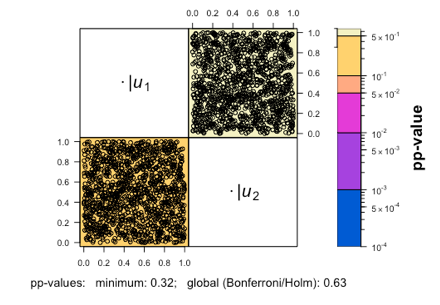
\includegraphics[width=100mm]{Rosenblatt}
  \caption{Rosenblatt plot - Student-t}
  \label{fig:plot data}
\end{figure}
The p-value looks reasonable. We will then simulate data from the selected copula.
\begin{lstlisting}
par(mfrow=c(1,2))
plot(Estimate_stocks1,Estimate_stocks2)
simSN = rCopula(length(Estimate_stocks1),t.Copula)
plot(simSN[,1],simSN[,2])
\end{lstlisting}
We obtain the two following plots.
\pagebreak
\begin{figure}[!ht]
 \center
  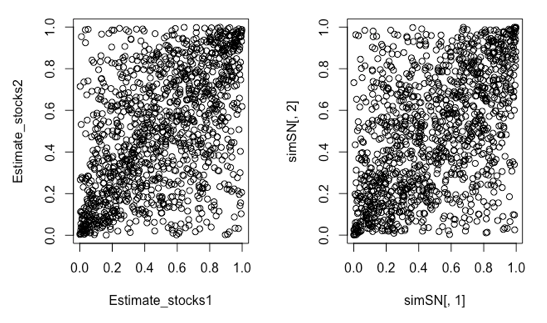
\includegraphics[width=100mm]{Scatterplots}
  \caption{Scatterplots Transformed/Simulated Data}
  \label{fig:plot data}
\end{figure}

It seems that our simulated data reflects the original transformed data quite well, especially because it has heavy right and left tails like our data.
We then look at the correlation between our two stocks in the original transformed data and the simulated one.
\begin{lstlisting}
cor(simSN[,1],simSN[,2])
cor(simSN[,1],simSN[,2],method="kendall")
cor(simSN[,1],simSN[,2],method="spearman")

cor(Estimate_stocks1,Estimate_stocks2)
cor(Estimate_stocks1,Estimate_stocks2,method="kendall")
cor(Estimate_stocks1,Estimate_stocks2,method="spearman")

\end{lstlisting}
We obtain the following results for the simulated  and original data: 
\\
\begin{table}[H]
    \centering
    \begin{tabular}{c|c|c}
            & Simulated Data    & Original data \\  \hline
    Correlation & 0.4933311         & 0.4884818\\ \hline
    Kendall     & 0.3559349         & 0.3502437\\ \hline
    Spearman    & 0.494149          & 0.4884818
    \end{tabular}
    \caption{Different correlation scores for simulated and original transformed data.}
    \label{tab:correlation_scores}
\end{table}


It looks that the copula reflects the correlation structure quite well.\\
Finally, we look at the derived univariate quantities and plot the ones of the original transformed data against the ones of the simulated data.
\begin{lstlisting}
USUN = sort(Estimate_stocks1+Estimate_stocks2,decreasing=FALSE)
simUSUN = sort(simSN[,1]+simSN[,2],decreasing=FALSE)
plot(USUN,simUSUN)
abline(0,1)
\end{lstlisting}
We obtain the following plot, that can be analyzed as a QQ-plot.
\begin{figure}[!ht]
 \center
  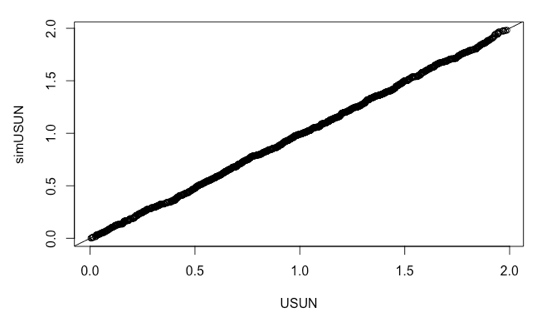
\includegraphics[width=100mm]{QQ-plot}
  \caption{QQ-plot}
  \label{fig:plot data}
\end{figure}

\subsection*{Summary}

First, we transformed our data to uniformly distributed observations on [0,1].
Then we tried to find a copula that fits our model. After trying different copula families we used the vinecopula library that helped us find the right parameters for the right copula: tcopula.
Finally, we used three methods to assess the goodness of fit of the copula. We used the Rosenblatt function to find the p-value that was pretty good and showed us that the copula is a good fit then we simulated our data using the same number of observations and the fitted copula and roughly compared the scatter plot of the log returns and our simulated data.
At the end, we plotted the sum of the marginals of our data
as a function of the sum of the marginals of the simulated one and ended up with a straight line that confirm out choice of tcopula.

\end{document}  